\documentclass[a4paper,12pt,abstracton,titlepage]{scrartcl}

\usepackage[french]{babel}
%\usepackage[T1]{fontenc}
\usepackage[utf8]{inputenc} % Umlaute, evtl. vom Betriebssystem abhaengig
\usepackage{lmodern}
\usepackage{pgfgantt}
\usepackage{titlesec}
\usepackage{float}
\usepackage{floatflt}
\usepackage{blindtext}
\usepackage{amsmath}
\usepackage{tabularx,url}
\usepackage[a4paper, left=2cm, textwidth=17cm, top=1.5cm]{geometry}
\usepackage{hyperref}
\usepackage{longtable}


\titleformat*{\section}{\large\bfseries}
\titleformat*{\subsection}{\large\bfseries}
\titleformat*{\subsubsection}{\large\bfseries}
\titleformat*{\paragraph}{\large\bfseries}
\titleformat*{\subparagraph}{\large\bfseries}

\renewcaptionname{french}{\figurename}{Fig.}

%\titlehead{Ulm University}
%\title{Title}
%\subject{Subject}
%\author{Author}
%\publishers{%
	%\rule{\textwidth}{0.4pt} \\
	%\vspace{0.5cm}
    %\normalfont\normalsize%
    %\parbox{0.9\linewidth}{%
    %    Abstract or Introduction
    %} \\
    %\vspace{0.5cm}
   	%\rule{\textwidth}{0.4pt}
%}

\renewcommand*\contentsname{Summary}

\begin{document}
%\maketitle

%%% begin costom title
{\Large\noindent \emph{ESIEE Paris}}

{\Large\noindent \emph{IGI-3008}}
\vspace{1cm}
\begin{center}
	{\huge \textbf{Cryptographie}
	\\
	\vspace{0.3cm}
	\large Léa MENERET, Fathima SAHADATTALY, Ulrike KULZER
	\\
	\vspace{0.2cm}
	\today}
\end{center}
%%% end custom title
\vspace{1cm}
%\maketitle
\tableofcontents

\setcounter{page}{1} % reset page counter to one for the first page, leave the title page out


\newpage
\section{Guide utilisateur}
\subsection{Introduction}
\subsubsection{En général}
La cryptographie est une technique utilisée pour rendre incompréhensible à autrui un message entre un expéditeur et un destinataire. Ce procédé a notamment été utilisé en période de guerre pour permettre des attaques surprises. 
Le principe est le suivant : L'expéditeur à partir d'une clé crypte son message et l'envoie au destinataire. Celui-ci possède aussi la clé qui va lui permettre ainsi de décrypter le message.

\subsubsection{Méthodes de cryptage}
La cryptographie est utilisée depuis l'Antiquité mais certaines de ces méthodes les plus abouties datent du 20e siècle. Il existe différents principes de cryptage plus ou moins compliqués tels que\\
\\
\begin{minipage}[t]{0.5\textwidth}
    \begin{itemize}
    \item \textit{le chiffre de César :}\\
    Ce procédé a été inventé lors de l'époque romaine par Jules César pour ses communications secrètes. En décalant l'alphabet par un entier donné chaque lettre est associée à une nouvelle lettre, ainsi on peut crypter le message initiale en remplaçant chaque lettre par la nouvelle lettre attribuée.
    \paragraph{}
    \item \textit{le chiffre de Vigenère :}\\
    Il a été inventé au 16e siècle par Blaise de Vigenère et est basé sur le tableau à droite. Une clé (un mot) est répétée et mis sous le message et de cette manière on peut trouver les lettres correspondantes à partir du tableau.\\
    Exemple:
%\footnote{https://fr.wikipedia.org/wiki/Chiffre_de_Vigen\%C3\%A8re}
    \end{itemize}
    \begin{center}
    \raggedleft
 	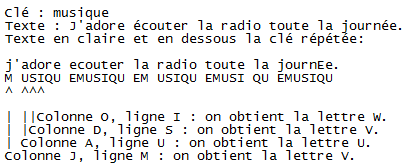
\includegraphics[height=3.4cm]{./Pictures/exempleVigenere_neuf.png}
 	%\caption{exemple du cryptage de Vigenère}
 	\label{exVig}
    \end{center} 
	
  \end{minipage} 
  \begin{minipage}[t]{0.4\linewidth}
    \raggedleft
    \strut\vspace*{-\baselineskip}\newline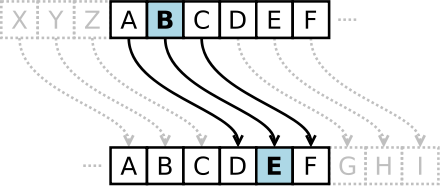
\includegraphics[width=0.9\linewidth]{./Pictures/chiffreCesar.png}
    %\caption{décalage de l'alphabet}
    \label{cesar}
    \paragraph{}
    \strut\vspace*{-\baselineskip}\newline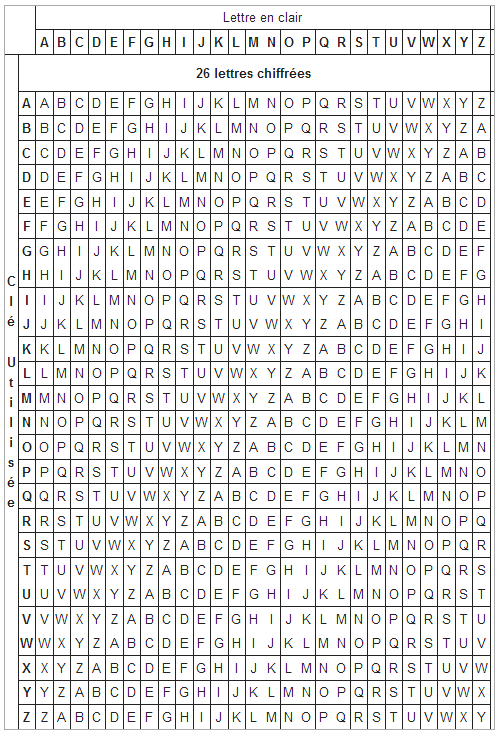
\includegraphics[width=0.9\linewidth]{./Pictures/tableauVigenere.png}
    %\caption{tableau de Vigenère}
    \label{tabVig}
  \end{minipage}

\begin{minipage}[t]{0.5\textwidth}
    \begin{itemize}
    \item \textit{celui de la machine Enigma :}\\
    L'Enigma est une machine de cryptographie inventée par Arthur Scherbius en 1919. Elle a été utilisée durant la Seconde Guerre mondiale pour la communication secrète entre les différentes unités de l'armée allemande.
La machine est constituée de cinq rotors dont un réflecteur, d'un clavier, d'un tableau de permutation et de lampes pour chaque lettre. Pour l'allumer il faut une batterie de 4,5 Volt.
Le principe est simple : Lorsqu'on appuie sur une lettre du clavier, un courant électrique va être envoyé au tableau de permutation dans lequel la lettre entrée est échangée avec une autre lettre si elles sont connectées. Puis il passera la première fois par les quatre rotors : Dans chacun des trois rotors au milieu il y a un décalage des lettres qui s'opère. À la fin les lettres sont permutées encore une fois dans le réflecteur qui les renvoie par les rotors au tableau de permutation ce qui permettra à une lampe correspondant à une lettre de s'allumer. Ainsi pour chaque lettre on relève la lettre codée, on obtient alors notre message crypté.\\
    \end{itemize}
  \end{minipage}
  \begin{minipage}[t]{0.5\linewidth}
    \raggedleft
    \strut\vspace*{-\baselineskip}\newline\newline\newline\includegraphics[width=0.9\linewidth]{./Pictures/enigma.jpg}
    %\caption{La machine Enigma}
    \label{enigma}
  \end{minipage}
  
\paragraph{}
\paragraph{}
\paragraph{}
\paragraph{}

\textit{Sites de référence :}
\begin{itemize}
\item \url{https://fr.wikipedia.org/wiki/Cryptographie}
\item \url{http://www.bibmath.net/crypto/}
\item \url{https://fr.wikipedia.org/wiki/Chiffrement_par_d\%C3\%A9calage}
\item \url{https://fr.wikipedia.org/wiki/Chiffre_de_Vigen\%C3\%A8re}
\item \url{https://fr.wikipedia.org/wiki/Enigma_(machine)}
\item photo d’Enigma:
Von William Warby from London, England - Enigma, CC BY 2.0,\\\url{https://commons.wikimedia.org/w/index.php?curid=46848023}\\
\end{itemize}

\newpage
\subsection{Fonctionnement du programme}

\subsubsection{Accueil et choix de la langue}
Pour exécuter notre programme, il est nécessaire de l'ouvrir avec le logiciel Pycharm, d'aller dans le fichier "`main\_module"' et d'appuyer sur "`run"' - "`run"' - "`run main\_module"'.
Les instructions du programme seront affichées dans la console qui s'ouvre en bas de l'interface comme montrés ci dessous :
\vspace{0.5cm}
\\
{\fbox{\parbox{\textwidth}{\raggedright
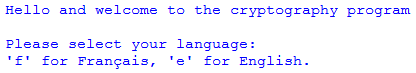
\includegraphics{./Pictures/interface/01_startScreen.png}}}
	\captionof{figure}{Écran d'accueil}
	\label{SP}
}
\vspace{0.5cm}
Vous venez d’entrer dans le programme Cryptographie, vous devez entrer la lettre ' f ' pour avoir les instructions en français et ' e ' pour les avoir en anglais.
Si la lettre entrée est ' e ', les prochaines instructions seront donc en anglais. \\
\\
Note: Vous retrouverez les mêmes interfaces en français.\\
\\
Une nouvelle fenêtre va ensuite apparaître :
\vspace{0.5cm}
\\
{\fbox{\parbox{\textwidth}{\raggedright
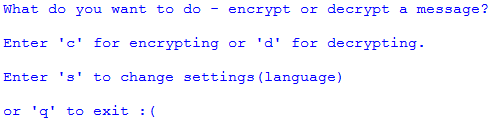
\includegraphics{./Pictures/interface/english/02_english_mainMenu.png}}}	%2
\captionof{figure}{Menu principal}
\label{EMM}
}
\vspace{0.5cm}

Le programme demande maintenant ce que vous voulez faire, vous devez entrer ' c ' si vous voulez que le programme crypte votre texte ou ' d ' si vous voulez qu'il le décrypte.
Si vous voulez changez de langue entrez ' s ' et si malheureusement vous voulez quitter le programme entrez ' q ' .\\
\newpage
Si la lettre entrée est ' s ' , une nouvelle fenêtre permettant de changer la langue va alors apparaitre.
\vspace{0.5cm}
\\
{\fbox{\parbox{\textwidth}{\raggedright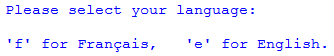
\includegraphics{./Pictures/interface/settingsDialogue.png}}}
\captionof{figure}{Paramètres}
\label{ESD}
}
\vspace{0.5cm}

Vous devez entrer la lettre ' f ' pour avoir les instructions en français et ' e ' pour les avoir en anglais.\\
Si la lettre entrée est ' f ' les prochaines instructions seront donc en français.\\
Vous reviendrez sur les instructions précédentes cette fois-ci en français.\\

\subsubsection{Crypter/Décrypter}
\vspace{0.5cm}
{\fbox{\parbox{\textwidth}{\raggedright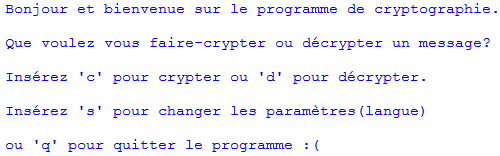
\includegraphics{./Pictures/interface/french/02_french_mainMenu.png}}}
\captionof{figure}{Menu principal}
\label{FMM}
}
\vspace{0.5cm}

Vous devez entrer ' c ' si vous voulez que le programme crypte votre texte ou ' d ' si vous voulez qu'il le décrypte.\\
Si vous voulez changer de langue entrez ' s ' et si malheureusement vous voulez quitter le programme entrez ' q ' .\\
\\
Si la lettre entrée est ' c ' , le programme va donc être servi pour le cryptage d'un texte.\\
Il existe trois méthodes par lesquelles le texte peut être crypté, nous allons donc détailler les différentes manières.


\newpage
\subsubsection{Choix du principe}
Si vous avez choisi de crypter votre texte, il vous faut maintenant choisir quelle méthode vous voulez utiliser, trois choix s'offrent à vous.

\vspace{0.5cm}
{\fbox{\parbox{\textwidth}{\raggedright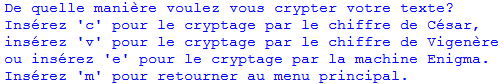
\includegraphics{./Pictures/interface/french/03_french_cryptage.png}}}
\captionof{figure}{Cryptage}
\label{FCr}
}
\vspace{0.5cm}

Vous devez entrer ' c ' si vous voulez que le programme crypte votre texte par la méthode du chiffre de César, ' v ' par la méthode du chiffre de Vigenère et enfin ' e ' par la méthode de la machine Enigma.\\
Si tout autre fois vous voulez retourner au menu principal, entrez ' m '.\\
\\
De la même manière, si à l'interface précédente vous aviez choisi le mode décryptage, vous allez devoir choisir la méthode par laquelle vous voulez décrypter votre texte. Les commandes pour choisir la méthode de décryptage sont alors les mêmes que pour un texte à crypter : ' c ' pour César, ' v ' pour Vigenère, ' e ' pour Enigma et ' m ' pour retourner au menu principal.

\vspace{0.5cm}
{\fbox{\parbox{\textwidth}{\raggedright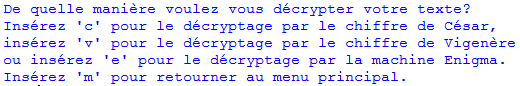
\includegraphics{./Pictures/interface/french/03_french_decryptage.png}}}
\captionof{figure}{Décryptage}
\label{FD}
}
\vspace{0.5cm}

Dans les deux cas vous pouvez consulter l'aide en entrant ' h ' qui vous rappellera les principes de cryptage utilisé pour les différentes méthodes César, Vigenère ou Enigma :

\vspace{0.5cm}
{\fbox{\parbox{\textwidth}{\raggedright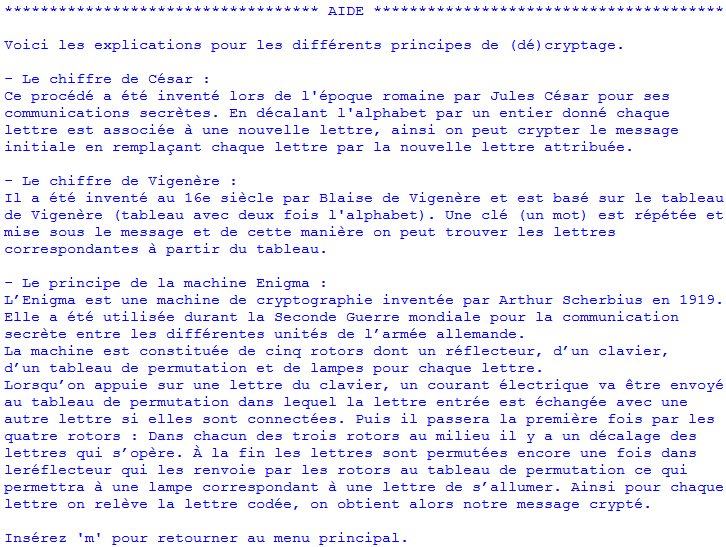
\includegraphics[width=\textwidth]{./Pictures/interface/french/08_french_helpMenu.png}}}
\captionof{figure}{Aide}
\label{FHM}
}
\vspace{1cm}

%\newpage
% diff. principes
% César
\textit{Le chiffre de César:}\\
Imaginons que vous ayez choisi de crypter ou décrypter votre texte par la méthode du chiffre de César, l'interface suivante apparaîtra :

\vspace{0.5cm}
{\fbox{\parbox{\textwidth}{\raggedright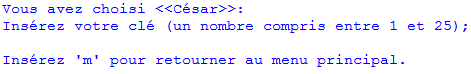
\includegraphics{./Pictures/interface/french/04_french_cesar.png}}}
\captionof{figure}{Le chiffre de César}
\label{FCe}
}
\vspace{0.5cm}

Vous devez maintenant choisir la clé à utiliser pour (dé)crypter votre texte. Cette clé doit être un nombre compris entre 1 et 25 et correspondra au décalage de l'alphabet lors du (dé)cryptage de chaque lettre.
Vous avez également la possibilité de retourner au menu principal en entrant ' m '.\\
\vspace{0.5cm}

\newpage
% Vigenère
\textit{Le chiffre de Vigenère:}\\
Si votre choix se porte sur le (dé)cryptage par la méthode du chiffre de Vigenère, vous verrez alors le message suivant :

\vspace{0.5cm}
{\fbox{\parbox{\textwidth}{\raggedright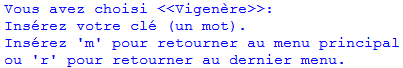
\includegraphics{./Pictures/interface/french/04_french_vigenere.png}}}
\captionof{figure}{Le chiffre de Vigenère}
\label{FV}
}
\vspace{0.5cm}

Vous devez maintenant entrer la clé que vous souhaitez utiliser. Cette clé doit être un mot composé uniquement de lettres (minuscules ou majuscules) sans espace ni tiret. 
Vous pouvez aussi entrer ' m ' si vous voulez retourner au menu principal.\\
\vspace{0.5cm}

% Enigma
\textit{La machine Enigma:}\\
Si vous avez sélectionné le (dé)cryptage par la méthode de la machine Enigma, le message suivant apparaîtra :

\vspace{0.5cm}
{\fbox{\parbox{\textwidth}{\raggedright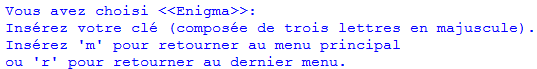
\includegraphics{./Pictures/interface/french/04_french_enigma.png}}}
\captionof{figure}{Le cryptage par la machine Enigma}
\label{FE}
}
\vspace{0.5cm}

Le programme attend de vous que vous entriez la clé de (dé)cryptage. Cette clé doit se présenter sous la forme de trois lettres majuscules.\\
Vous avez toujours, comme précédemment la possibilité de retourner au menu principal en entrant ' m '.
\vspace{1cm}

Quelle que soit la méthode de (dé)cryptage choisie vous serez confronté au message suivant qui vous indique d'entrer le texte à traiter. Il est important de savoir que dans le texte tous les caractères spéciaux seront normalisés et les chiffres et signes de ponctuation seront enlevés.\\
% original :Ce texte ne devra comporter que des lettres minuscules, majuscules, avec ou sans accents. Aucun chiffre ou aucune ponctuation ne pourra être entrée.\\
\\
À ce stade vous pouvez aussi entrer ' m ' pour retourner au menu principal.

\vspace{0.5cm}
{\fbox{\parbox{\textwidth}{\raggedright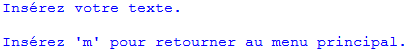
\includegraphics{./Pictures/interface/french/05_french_insertText.png}}}
\captionof{figure}{Entrée du texte}
\label{FIT}
}
\vspace{0.5cm}

\newpage
Enfin le programme s'exécute pour effectuer l'opération que vous lui avez demandé, et l'un des message suivant apparaîtra suivi de votre texte crypté ou décrypté.

\vspace{0.5cm}
{\fbox{\parbox{\textwidth}{\raggedright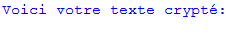
\includegraphics{./Pictures/interface/french/06_french_cryptage_showText.png}}}
\captionof{figure}{Affichage du texte crypté}
\label{FSCT}
\vspace{0.7cm}
\fbox{\parbox{\textwidth}{\raggedright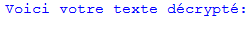
\includegraphics{./Pictures/interface/french/06_french_decryptage_showText.png}}}
\captionof{figure}{Affichage du texte décrypté}
\label{FSDT}
}
\vspace{0.7cm}

Sous le texte (dé)crypté il s'affichera la phrase suivante:

\vspace{0.5cm}
{\fbox{\parbox{\textwidth}{\raggedright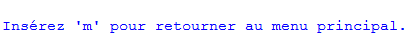
\includegraphics{./Pictures/interface/french/99_french_continue.png}}}
\captionof{figure}{Affichage du texte crypté}
\label{FrCon}
\vspace{0.7cm}

Il faut insérer ' m ' pour retourner au menu principal.\\

À partir de cela vous pouvez choisir, si vous voulez continuer ou quitter le programme (voir \ref{FMM}).\\

Si ensuite la lettre entrée est ' q ', le message de fin s'affichera:

\vspace{0.5cm}
{\fbox{\parbox{\textwidth}{\raggedright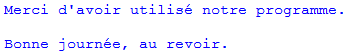
\includegraphics{./Pictures/interface/french/07_french_quitMessage.png}}}		%23
\captionof{figure}{Sortie du programme}
\label{FSQM}
}


% ########### guide de maintenance

\newpage
\section{Guide de maintenance}
\subsection{Fonctionnalité}
\subsubsection{En général}
\begin{itemize}
\item Quand l’utilisateur lance le programme on lui demande de choisir la langue, soit français, soit anglais.
\item Notre programme va proposer à l’utilisateur trois façons différentes de (dé)crypter un texte de complexité croissante et demander une clé.
\item Les différentes manières sont le principe du chiffre de César, du chiffre de Vigenère et de la machine Enigma.
\end{itemize}

\subsubsection{Différents états du programme}
Les différents états du programme sont représentés dans le diagramme ci-dessous. Dès que le programme est lancé, il est généralement toujours dans un état en attendant des saisies de l'utilisateur. La seule exception est l'état en cryptant ou décryptant.
Sur les flèches on peut voir ce qu'il faut faire pour accéder à un autre état, soit le précédent, soit le suivant.
Avant que le programme est fermé, il affichera un petit message de remerciement.\\

\begin{figure}[tpbh]
	\centering
  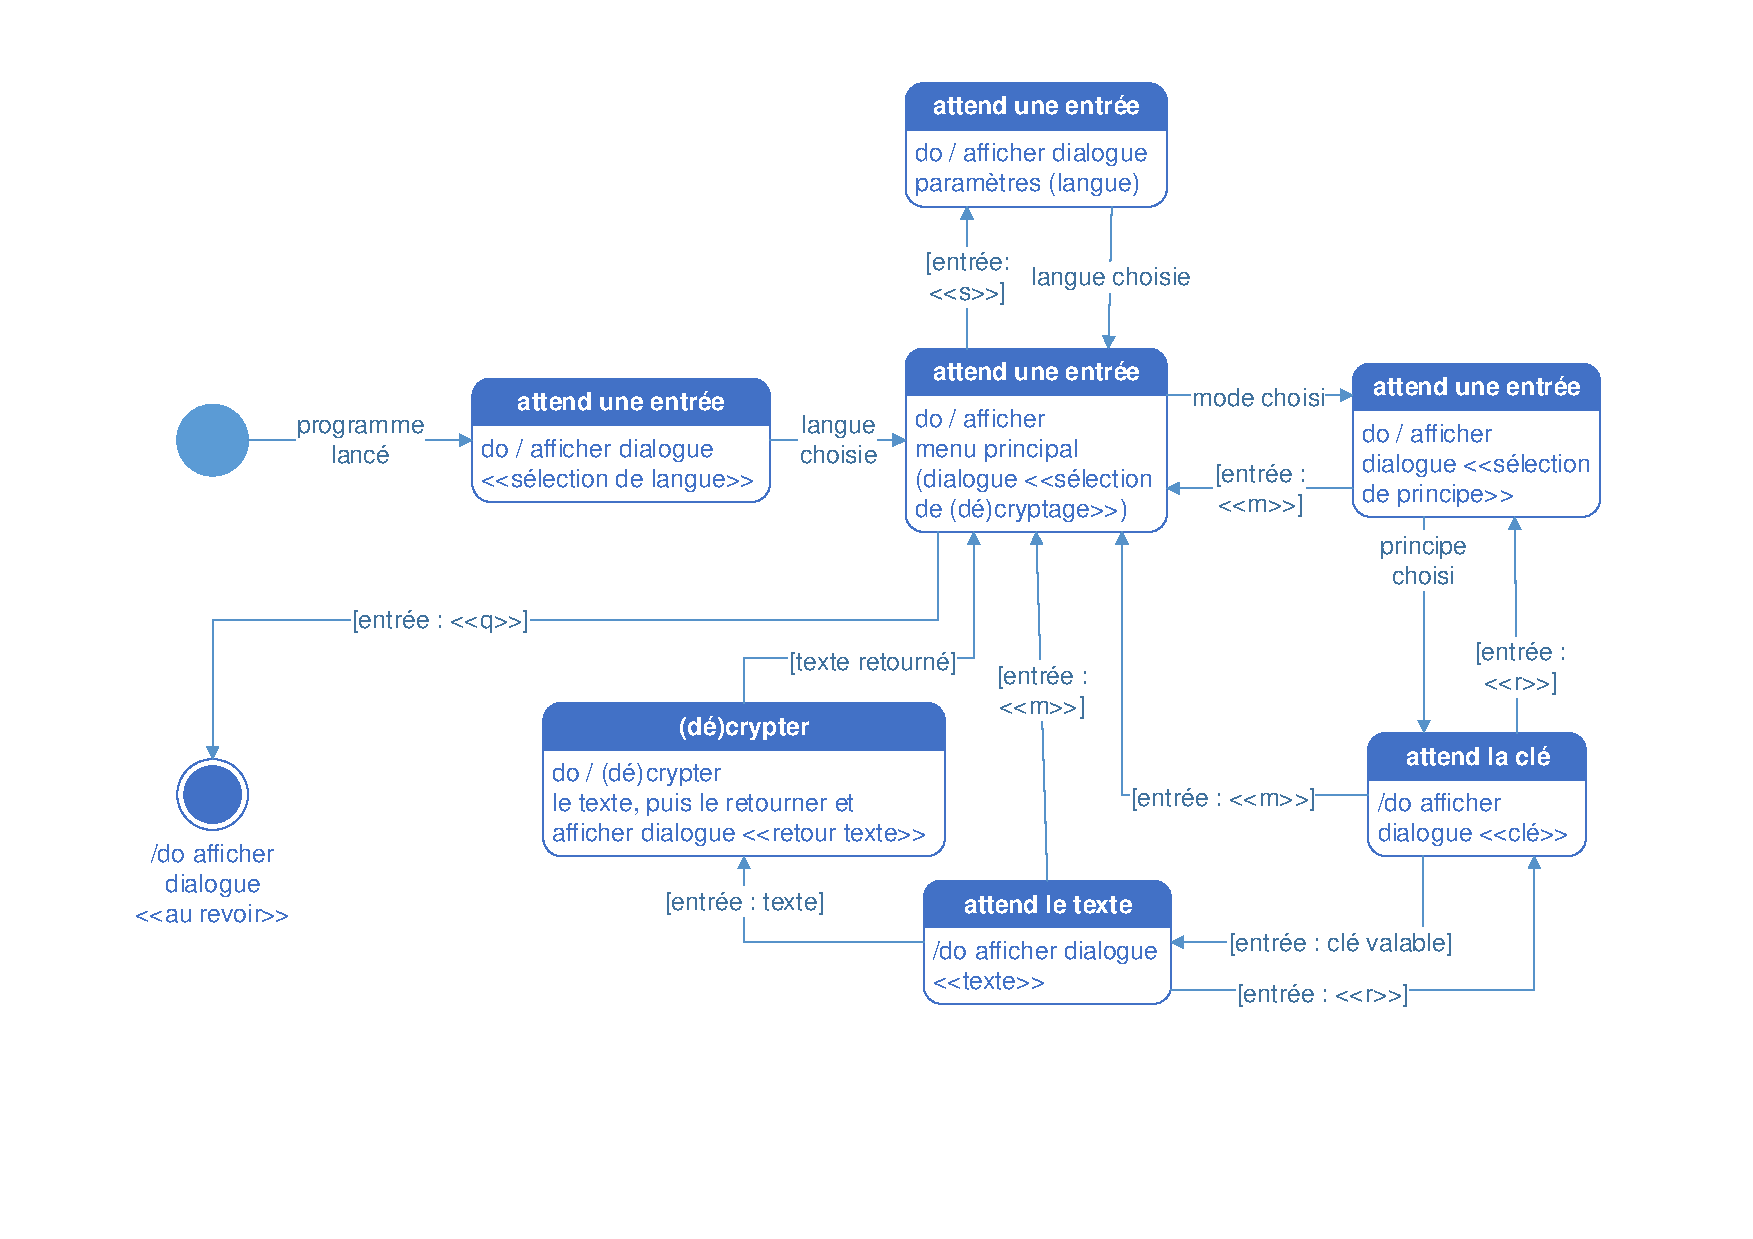
\includegraphics[width=\textwidth, trim=20mm 25mm 25mm 13mm, clip]{./Diagrammes/diagrammeDesEtats.pdf}
  %TRIM = LINKS UNTEN RECHTS OBEN
  \captionof{figure}{Diagramme états-transitions du programme}
	\label{img:etats}
\end{figure}


\newpage
\subsubsection{En détail et coupé en modules}
\begin{itemize}
\item \textit{Avant de commencer le (de)cryptage :}\\
On va créer une méthode qui formatera le texte (enlever les accents, les caractères spéciaux, les signes de ponctuation et les espaces, puis mettre tout en majuscule).\\
% César
\item \textit{(Dé)Cryptage César :}\\
On compte transformer les lettres du texte en nombres par le système unicode, ensuite on additionne la clé (nombre) aux nombres obtenus par le système.On reconvertit alors les lettres en caractères et retourne le texte.
Pour le décryptage, il suffit de soustraire au lieu d'additionner.\\
% Vigenère
\item \textit{(Dé)Cryptage Vigenère :}\\
Dans un premier temps on crée une matrice de 26 x 26 lettres contenant l’alphabet représentant le tableau de Vigenère et une matrice à deux lignes pour le texte et la clé. Dans un deuxième temps on prend le texte et on insère tour à tour les caractères individuels dans la première ligne de la matrice et la clé dans la deuxième. Chaque lettre du texte doit être attribuée à un caractère de la clé (mot) ce qui est permis en répétant le mot tant qu’ils restent des lettres du texte.
Le cryptage est fait caractère par un caractère. Pour trouver la lettre cryptée on regarde en premier la lettre du texte et on cherche la colonne de la matrice qui appartient à la lettre et on la mémorise. Par la suite on considère le caractère de la clé auquel la lettre du texte est attribuée et on cherche la ligne de la matrice qui appartient au caractère. Dès qu’on a trouvé les deux, la lettre de la matrice qui est enregistré sur cette case est la lettre cryptée laquelle est mémorisée dans une chaîne de caractère. Lorsqu’on a crypté toutes les lettres du texte, on retourne la chaîne de caractère qui est le texte crypté.
Pour le décryptage, on possède la matrice à deux lignes avec le texte crypté sur une ligne et la clé répétée sur l’autre. Pour chaque lettre du texte crypté, on parcourt dans le tableau de Vigenère (matrice) la ligne correspondant à la lettre de la clé répétée et lorsqu’on  trouve la lettre cryptée cherchée on remonte la ligne pour obtenir le caractère décrypté correspondant à cette lettre. De la même manière que pour le cryptage on mémorise les lettres obtenues dans une chaîne de caractère ce qui permet d’avoir au final le message décrypté.\\
% Enigma
\item \textit{(Dé)Cryptage Enigma :}\\
Pour commencer nous créons cinq listes : La première correspond au tableau de permutation, les trois suivantes aux rotors au milieu et la dernière au réflecteur. Au début de la programmation on choisit un décalage fixe ; si possible on essayera plus tard de changer le décalage automatiquement.
Pour les connecteurs, il y en aura dix ainsi 20 lettres seront connectées entre elles et six qui ne le seront pas. Nous allons créer une fonction qui, si la lettre est connectée, va retourner la lettre associée.
On appelle ensuite des fonctions qui exécutent les décalages au niveau des trois rotors et après on utilise la fonction correspondant au réflecteur pour permuter les lettres. On repasse finalement à nouveau par les rotors et on obtient une certaine lettre. Si la lettre est connectée à une autre, on retourne l’autre lettre, sinon on garde la même, celle-ci est alors la lettre (dé)cryptée.\\
\end{itemize}

\newpage
\subsubsection{Structure du programme}
% diagrammme\\

\begin{minipage}[c]{\textwidth}
\centering
    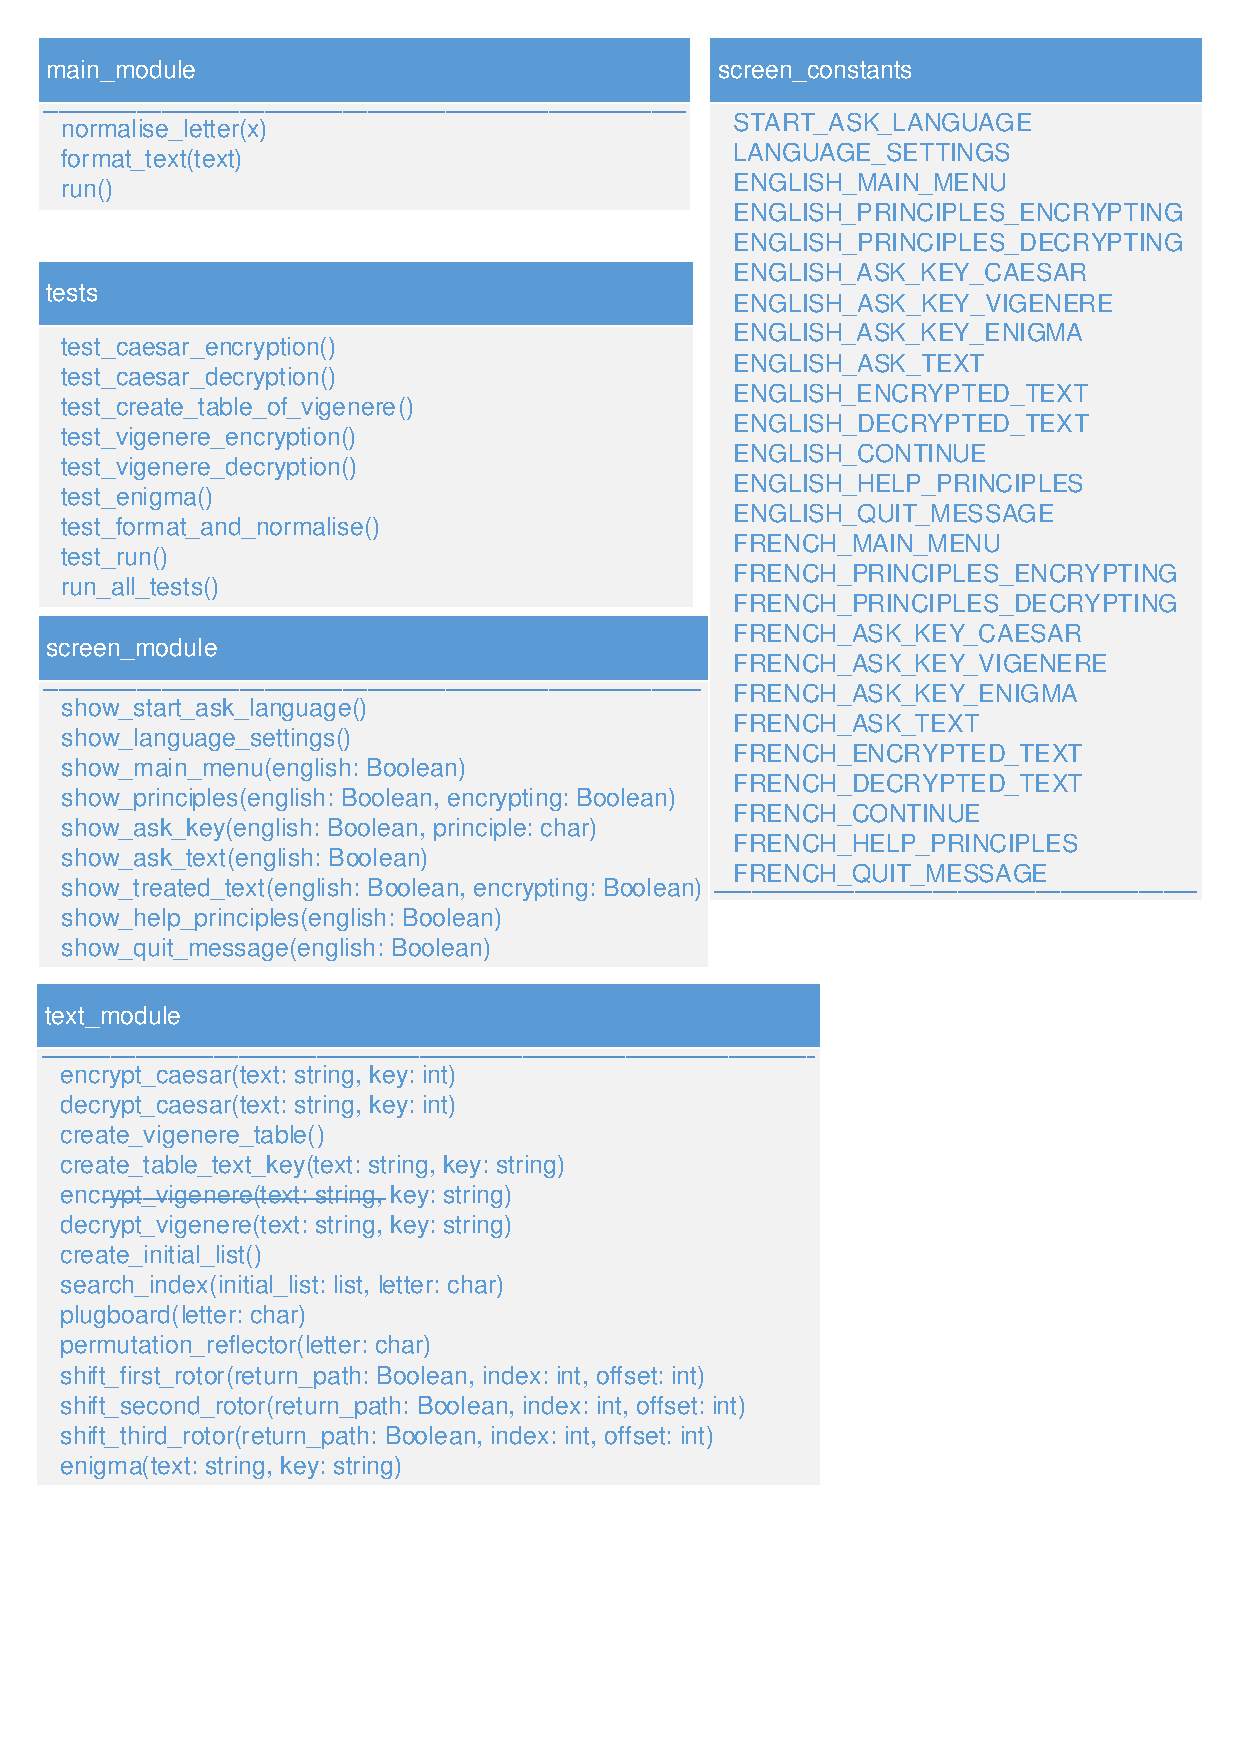
\includegraphics[width=\textwidth, trim=1mm 40mm 1mm 1mm, clip]{./Diagrammes/diagrammeDeStructure_main_modules.pdf}
    %TRIM = LINKS UNTEN RECHTS OBEN
    \captionof{figure}{Structure du programme en modules}
    \label{img:structure}
\end{minipage}


\newpage
\subsubsection{Explications des modules, constantes et fonctions}
\textbf{Explications du module \textit{screen\_constants} :}\\
Ce module contient toutes les constantes nécessaires pour le screen\_module, c'est-à-dire tous les textes de l'interface utilisateur.
\vspace{0.3cm}

\begin{itemize}
\item \textbf{START\_ASK\_LANGUAGE}:\\
dialogue de démarrage (voir fig. \ref{SP})\\
\item \textbf{LANGUAGE\_SETTINGS}:\\
dialogue des paramètres de langue (voir fig. \ref{ESD})\\
\item \textbf{ENGLISH\_MAIN\_MENU} et \textbf{FRENCH\_MAIN\_MENU}:\\
menu principal (voir fig. \ref{EMM} et \ref{FMM})\\
\item \textbf{ENGLISH\_PRINCIPLES\_ENCRYPTING} et\\
\textbf{FRENCH\_PRINCIPLES\_ENCRYPTING}:\\
dialogue de sélection du principe de cryptage (voir fig. \ref{FCr})\\
\item \textbf{ENGLISH\_PRINCIPLES\_DECRYPTING} et\\
\textbf{FRENCH\_PRINCIPLES\_DECRYPTING}:\\
dialogue de sélection du principe de décryptage (voir fig. \ref{FD})\\
\item \textbf{ENGLISH\_ASK\_KEY\_CAESAR} et \textbf{FRENCH\_ASK\_KEY\_CAESAR}:\\
dialogue de demande de la clé pour (dé)crypter par César (voir fig. \ref{FCe})\\
\item \textbf{ENGLISH\_ASK\_KEY\_VIGENERE} et \textbf{FRENCH\_ASK\_KEY\_VIGENERE}:\\
dialogue de demande de la clé pour (dé)crypter par Vigenère (voir fig. \ref{FV})\\
\item \textbf{ENGLISH\_ASK\_KEY\_ENIGMA} et \textbf{FRENCH\_ASK\_KEY\_ENIGMA}:\\
dialogue de demande de la clé pour (dé)crypter par Enigma (voir fig. \ref{FE})\\
\item \textbf{ENGLISH\_ASK\_TEXT} et \textbf{FRENCH\_ASK\_TEXT}:\\
dialogue de demande du text à (dé)crypter (voir fig. \ref{FIT})\\
\item \textbf{ENGLISH\_ENCRYPTED\_TEXT} et \textbf{FRENCH\_ENCRYPTED\_TEXT}:\\
dialogue du texte crypté (voir fig. \ref{FSCT})\\
\item \textbf{ENGLISH\_DECRYPTED\_TEXT} et \textbf{FRENCH\_DECRYPTED\_TEXT}:\\
dialogue du texte décrypté (voir fig. \ref{FSDT})\\
\item \textbf{ENGLISH\_CONTINUE} et \textbf{FRENCH\_CONTINUE}:\\
dialogue du pour continuer après avoir reçu le text (dé)crypté (voir fig. \ref{FrCon})\\
\item \textbf{ENGLISH\_HELP\_PRINCIPLES} et \textbf{FRENCH\_HELP\_PRINCIPLES}:\\
dialogue d'aide (voir fig. \ref{FHM})\\
\item \textbf{ENGLISH\_QUIT\_MESSAGE} et \textbf{FRENCH\_QUIT\_MESSAGE}:\\
message de sortie (voir fig. \ref{FSQM})\\
\end{itemize}

%\newpage
% screen_module
\textbf{Explications du module \textit{screen\_module:}}\\
Ce module est responsable de l'interface utilisateur, c'est-à-dire il montre le bon texte dans la langue choisie.
\vspace{0.3cm}

\begin{longtable}{ll} 
\textbf{show\_start\_ask\_language} & (ligne 8) \\     
Déclaration & show\_start\_ask\_language()\\
Rôle & demande à l'utilisateur la langue qu'il veut utiliser au début\\
 & du programme\\
Paramètre & aucun\\
Retour & la chaîne de caractère choisie par l'utilisateur:\\
 & ' f ' pour le français\\
 & ' e ' pour l'anglais\\
Appelé par & run()\\
Appelle & aucun\\
%\end{tabular}
%\vspace{0.5cm}
\cr 
\cr
%\begin{tabular}[t]{ll} 
\textbf{show\_language\_settings} & (ligne 18)\\
Déclaration & show\_language\_settings()\\
Rôle & demande à l'utilisateur la langue qu'il veut utiliser au cours\\
 & du programme\\
Paramètre & aucun\\
Retour & la chaîne de caractère choisie par l'utilisateur:\\
 & ‘ f ’ pour le français\\
 & ‘ e ‘ pour l'anglais\\
Appelé par &  run()\\
Appelle & aucun\\
%\end{tabular}
%\vspace{0.5cm}
\cr 
\cr
%\begin{tabular}[t]{ll} 
\textbf{show\_main\_menu} & (ligne 28)\\
Déclaration & show\_main\_menu(english)\\
Rôle & demande à l'utilisateur ce qu'il veut utiliser la fonction cryptage\\
 & ou décryptage du programme\\
Paramètre & english: booléen \\
 & True si la langue choisie est l'anglais\\
 & False si la langue choisie est le français\\
Retour & la chaîne de caractère choisie par l'utilisateur:\\
 & 'c' pour cryptage\\
 & 'd' pour décryptage\\
 & 's' pour changer de langue\\
 & 'q' pour quitter le programme\\
Appelé par & run()      (attention à vérifier)\\
Appelle & aucun\\
%\end{tabular}
%\vspace{0.5cm}
\cr 
\cr
\cr 
\cr 
\cr
\cr
%\begin{tabular}[t]{ll} 
\textbf{show\_principles} & (ligne 50)\\
Déclaration & show\_principles(english, encrypting)\\
Rôle & demande à l'utilisateur la méthode qu'il veut utiliser\\
 & pour (dé)crypter\\
Paramètre & english: booléen\\
 & True si la langue choisie est l'anglais\\
 & False si la langue choisie est le français\\
 & encryption: booléen\\
 & True si l'utilisateur veut crypter\\
 & False s'il veut décrypter\\
Retour & la chaîne de caractère choisie par l'utilisateur:\\
 & 'c' pour la méthode César\\
 & 'v' pour la méthode Vigenère\\
 & 'e' pour la méthode de la machine Enigma\\
 & 'm' pour retourner au menu principal\\
Appelé par & run()       (attention à vérifier)\\
Appelle & aucun\\
%\end{tabular}
%\vspace{0.5cm}
\cr 
\cr
%\begin{tabular}[t]{ll} 
\textbf{show\_ask\_key} & (ligne 81)\\
Déclaration & show\_ask\_key(english, principle)\\
Rôle & demande à l'utilisateur la clé pour la méthode qu'il veut utiliser\\
 & pour (dé)crypter\\
Paramètre & english: booléen\\
 & True si la langue choisie est l'anglais\\
 & False si la langue choisie est le français\\
 & principle: char\\
 & ' c ', ' v ' ou ' e ' selon la méthode de (dé)cryptage qu'il a choisi\\
Retour & la clé ou \\
 & ' m ' pour retourner au menu principal\\
Appelé par & run()      (attention à vérifier)\\
Appelle & aucun\\
%\end{tabular}
%\vspace{0.5cm}
\cr 
\cr
%\begin{tabular}[t]{ll} 
\textbf{show\_ask\_text} & (ligne 115)\\
Déclaration & show\_ask\_text(english)\\
Rôle & demande à l'utilisateur le texte qu'il veut (dé)crypter\\
Paramètre & english: booléen\\
 & True si la langue choisie est l'anglais\\
 & False si la langue choisie est le français\\
Retour & la clé ou\\
 & 'm' pour retourner au menu principal\\
Appelé par & run()      (attention à vérifier)\\
Appelle & aucun\\
%\end{tabular}
%\vspace{0.5cm}
\cr 
\cr
\cr
\cr
%\begin{tabular}[t]{ll} 
\textbf{show\_treated\_text} & (ligne 135)\\
Déclaration & show\_treated\_text(english, encrypting)\\
Rôle & retourne le message d'affichage du texte (dé)crypté\\
Paramètre & english: booléen \\
 & True si la langue choisie est l'anglais\\
 & False si la langue choisie est le français\\
 & encryption: booléen\\
 & True si l'utilisateur veut crypter\\
 & False s'il veut décrypter\\
Retour & le message d'affichage du texte (dé)crypté\\
Appelé par & run()   (attention à vérifier)\\
Appelle & aucun\\
%\end{tabular}
%\vspace{0.5cm}
\cr 
\cr
%\begin{tabular}[t]{ll} 
\textbf{show\_help\_principles} & (ligne 162)\\
Déclaration & show\_help\_principles(english)\\
Rôle & Affiche une aide dans laquelle le principe\\
 & de chaque méthode est expliquée\\
 & demande la saisie de ' m ' pour retourner au menu principal\\
Paramètre & english: booléen \\
 & True si la langue choisie est l'anglais\\
 & False si la langue choisie est le français\\
Retour & ' m ' \\
Appelé par & run()       (attention à vérifier)\\
Appelle & aucun\\
%\end{tabular}
%\vspace{0.5cm}
\cr 
\cr
%\begin{tabular}[t]{ll} 
\textbf{show\_quit\_message} & (ligne 180)\\
Déclaration & show\_quit\_message(english)\\
Rôle & Affiche un message de fin d'utilisation du programme\\
Paramètre & english: booléen \\
 & True si la langue choisie est l'anglais\\
 & False si la langue choisie est le français\\
Retour & aucun\\
Appelé par & run()     (attention à vérifier)\\
Appelle & aucun\\
\end{longtable}
\vspace{0.5cm}


\newpage
% text_module
\textit{\textbf{text\_module:}}\vspace{0.2cm}
\begin{itemize}
\item \textbf{encrypt\_caesar(text, key)}:\\
crypte le texte formaté par la méthode César\\
\item \textbf{decrypt\_caesar(text, key)}:\\
décrypte le texte formaté par la méthode César\\
\item \textbf{create\_vigenere\_table()}:\\
TODO\\
\item \textbf{create\_table\_text\_key(text, key)}:\\
TODO\\
\item \textbf{encrypt\_vigenere(text, key)}:\\
crypte le texte formaté par la méthode Vigenère\\
\item \textbf{decrypt\_vigenere(text, key)}:\\
décrypte le texte formaté par la méthode Vigenère\\
\item \textbf{create\_initial\_list()}:\\
TODO\\
\item \textbf{search\_index(initial\_list, letter)}:\\
cherche l'indice d'une lettre donnée dans une liste donnée\\
\item \textbf{plugboard(letter)}:\\
modélise le tableau de permutation, 10 lettres sont associées à dix autres lettres. Si la lettre donnée est associée à une autre lettre celle-ci va être retournée. Il y a six lettres qui ne sont associées à aucune autre lettre.\\
\item \textbf{permutation\_reflector(letter: char)}:\\
modélise le réflecteur ; même principe que plugboard(letter), mais cette fois-ci toutes les lettres sont associées à une autre lettre\\
\item \textbf{shift\_first\_rotor(letter: char)}:\\
modélise le premier rotor, exécute le décalage des lettres par indices et retourne la lettre correspondante\\
\item \textbf{shift\_second\_rotor(letter: char)}:\\
modélise le deuxième rotor, exécute le décalage des lettres par indices et retourne la lettre correspondante\\
\item \textbf{shift\_third\_rotor(letter: char)}:\\
modélise le troisième rotor, exécute le décalage des lettres par indices et retourne la lettre correspondante\\
\item \textbf{enigma(text, key)}:\\
(dé)crypte le texte formaté par la méthode Enigma\\
\end{itemize}\vspace{0.3cm}


% main_module
\textit{\textbf{main\_module:}}\vspace{0.2cm}
\begin{itemize}
\item \textbf{normalise\_letter(x)}:\\
normalise une lettre si elle est par exemple un caractère spécial\\
\item \textbf{format\_text(text)}:\\
formate le texte, c'est-à-dire le texte donné est mis en majuscules, les virgules, espaces, chiffres, symboles, etc. sont enlevés et les caractères spéciaux sont normalisés\\
\item \textbf{run()}:\\
démarre le programme et contrôle son déroulement\\
\end{itemize}\vspace{0.3cm}


% tests
\textit{\textbf{tests:}}\vspace{0.2cm}
\begin{itemize}
\item \textbf{test\_caesar\_encryption()}:\\
TODO\\
\item \textbf{test\_caesar\_decryption()}:\\
TODO\\
\item \textbf{test\_create\_table\_of\_vigenere()}:\\
TODO\\
\item \textbf{test\_vigenere\_encryption()}:\\
TODO\\
\item \textbf{test\_vigenere\_decryption()}:\\
TODO\\
\item \textbf{test\_enigma()}:\\
TODO\\
\item \textbf{test\_format\_and\_normalise()}:\\
TODO\\
\item \textbf{test\_run()}:\\
TODO\\
\item \textbf{run\_all\_tests()}:\\
TODO\\
\end{itemize}





\section{Annexe: Code du programme}






%\begin{floatingfigure}[l]{5.3cm}
%	\includegraphics[width=0.25\textwidth]{./Bilder/2venn.png}
%	\caption{Prinzip der additiven Farbmischung}
%	\label{venn}
%\end{floatingfigure}


%\par
%\vspace{2em}
%\vspace{1em}

% "`Standard Definition Television"', HDTV für "`High Definition Television'".



%\begin{tabular}[t]{lr}
%Naher Osten & 65\%\\
%Lateinamerika & 13\%\\
%\end{tabular}\\

%\begin{itemize}
%\item \blindtext
%\item \blindtext
%\end{itemize}
%\begin{enumerate}
%\item \blindtext
%\item \blindtext
%\end{enumerate}
%\begin{description}
%\item [Ant] \blindtext
%\item [Elephant] \blindtext

%\textbf{greatest} 
%\underline{science} 
%\textbf{\textit{accident}}.


\end{document}




% LABEL UNTER CAPTION

